\section{Case Study 1: Unnamed Aerial Vehicle}

\subsection{Model A}

\begin{figure}[!htb]
    \centering
    \caption[Forces normalized obtained from the neural network 1]{Forces normalized obtained from the neural network 1. Comparison is made from the results predicted from the neural network and the normalized preprocessing data, both for input and output data.}
    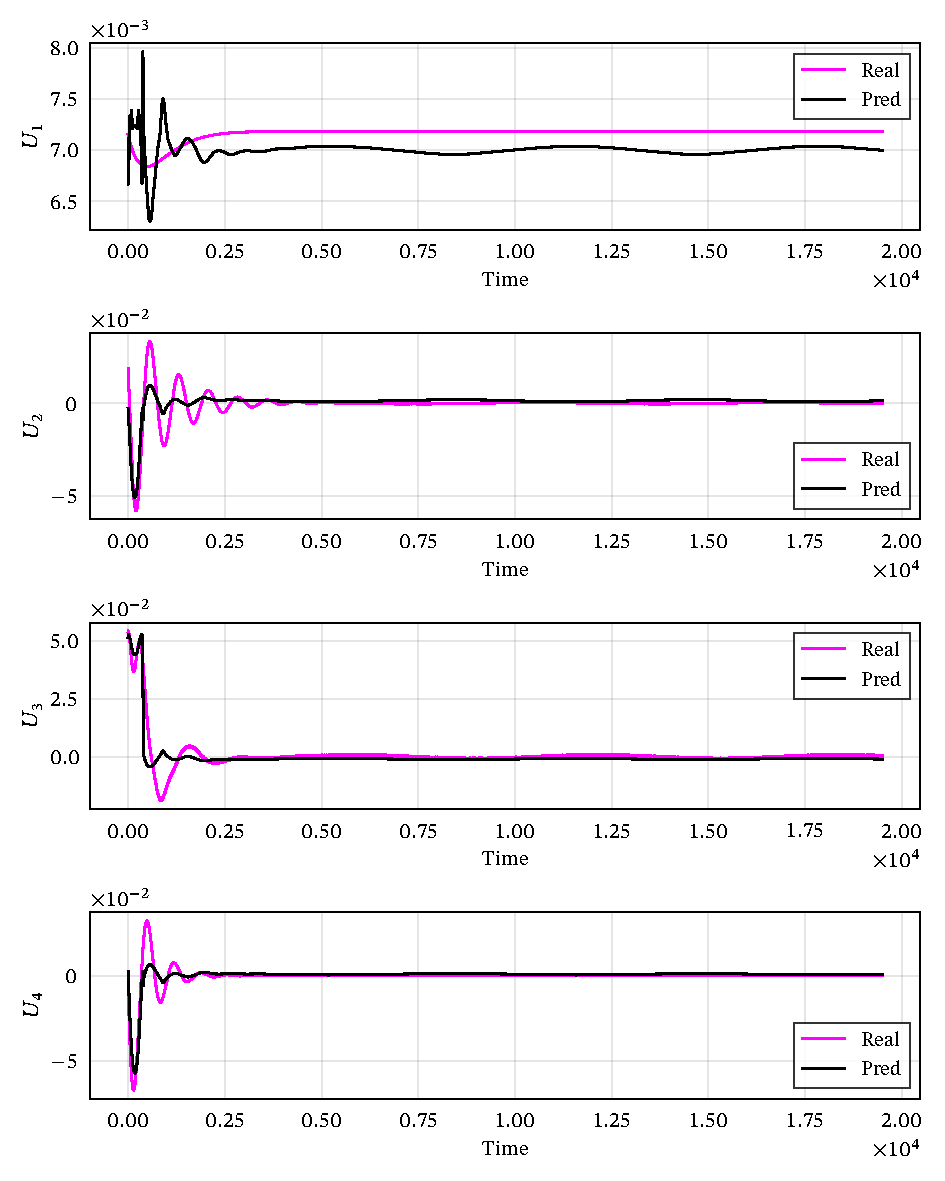
\includegraphics{figures/4results/uav/forces_normalized.pdf}

    {\footnotesize Source: prepared by the author.}
    \label{fig:forces_normalized}
\end{figure}

\begin{figure}[!htb]
    \centering
    \caption[Forces denormalized obtained from the combination of neural network 1 and 2]{Forces denormalized obtained from the combination of neural network 1 and 2. Comparison is made from the results predicted from the combination of both neural network and the raw data got from the white box parametric model.}
    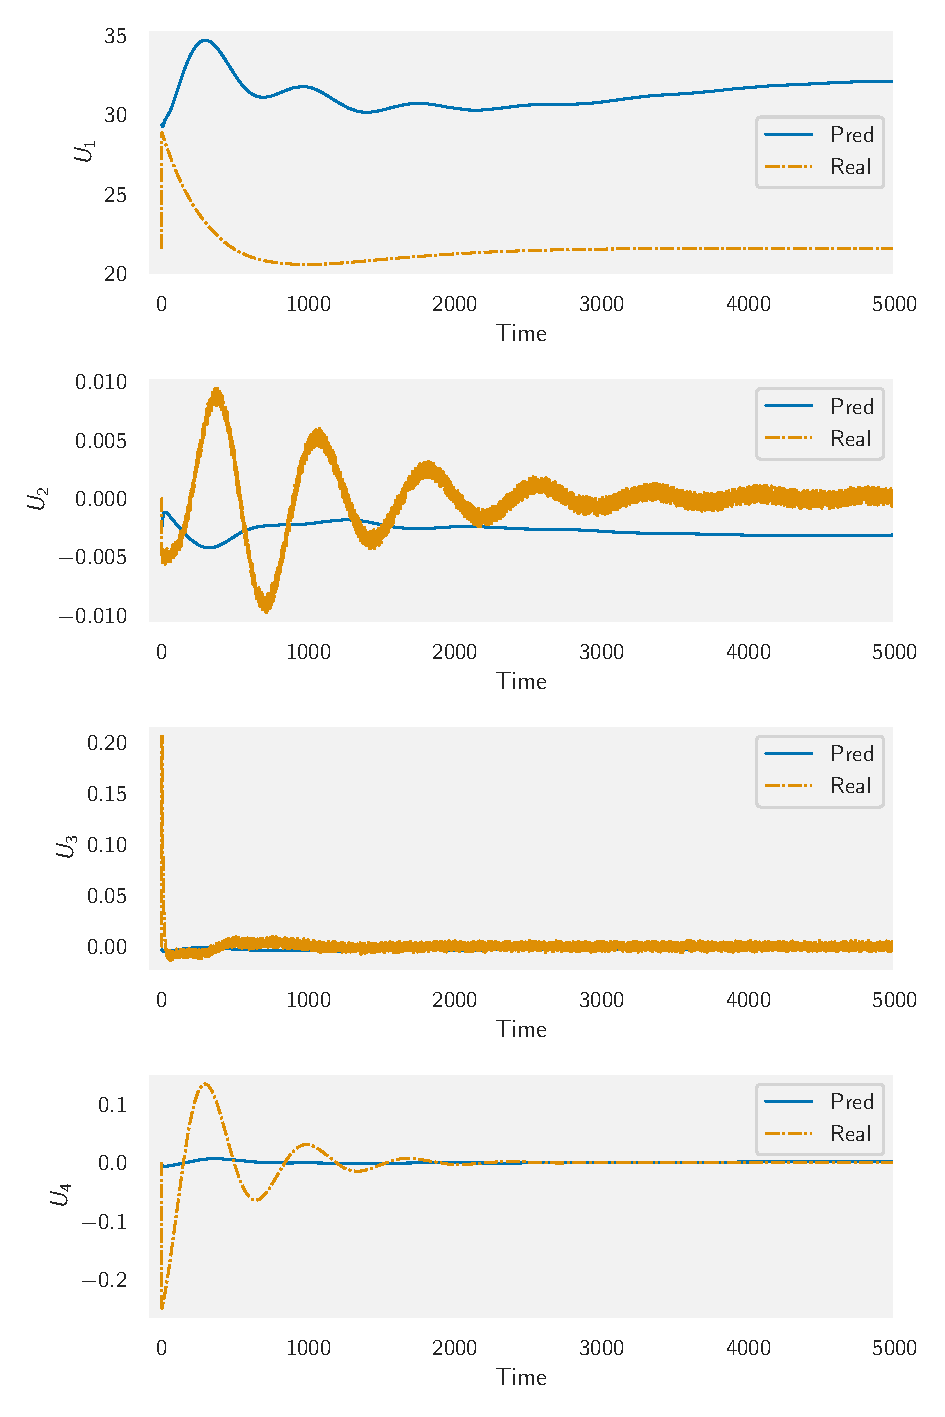
\includegraphics{figures/4results/uav/forces_denormalized.pdf}

    {\footnotesize Source: prepared by the author.}
    \label{fig:forces_denormalized}
\end{figure}

\begin{figure}[!htb]
    \centering
    \caption[Forces denormalized obtained from the combination of neural network 1 and 2 plus correction]{ denormalized obtained from the combination of neural network 1 and 2 plus correction. Comparison is made from the results predicted from the combination of both neural network and the raw data got from the white box parametric model with a correction for \(U_1\).}
    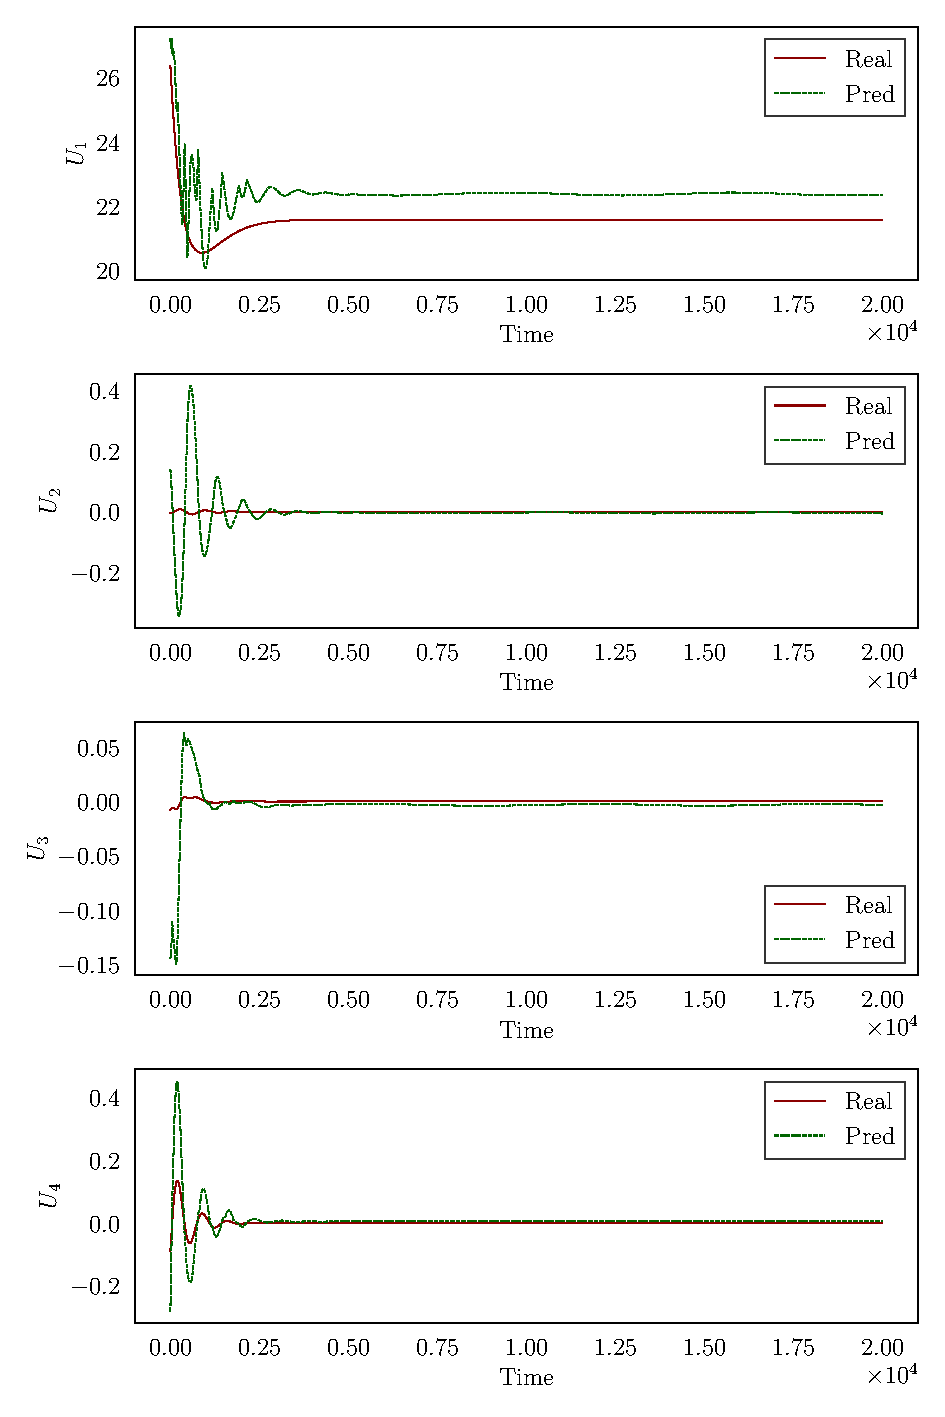
\includegraphics{figures/4results/uav/forces_denormalized_correction.pdf}

    {\footnotesize Source: prepared by the author.}
    \label{fig:forces_denormalized_correction}
\end{figure}

